\subsection{因子整环的刻画}

给定一个环 A，我们需要考虑以下条件：

\begin{enumerate}
\def\labelenumi{(\Alph{enumi})}
\setcounter{enumi}{12}
\tightlist
\item
  A 的整主理想的每个非空族都有一个极大元。
\end{enumerate}

定理1. 设 A 是整环。以下条件等价：

\begin{enumerate}
\def\labelenumi{(\alph{enumi})}
\item
  A 是因子整环；
\item
  A 的非零分式主理想的有序群是若干个同构于 Z 的群的直和（按乘积序排列）；
\item
  条件 (M) 成立，且 \(\mathbf{A}\) 的两个主理想的交是主理想；
\item
  条件 (M) 成立，且对于每个极值元 \(p\)（属于 \(\mathbf{A}\)），理想 \(\mathbf{A}p\) 是素理想；
\item
  A 是 Krull 整环，且每个高度为1的素理想都是主理想。
\end{enumerate}

我们把 K 记为 A 的分式域，把 \(\mathcal{P}^{*}\)（或 \(\mathcal{P}^{*}(A)\)）记为 A 的非零分式主理想的有序群。证明将通过证明以下蕴含来完成：

\pandocbounded{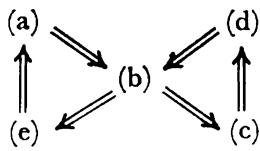
\includegraphics[keepaspectratio]{images/part003_cb91c25e.jpg}}

先证明 (a) 蕴含 (b)；若 A 是因子整环，则 \(P^{*}\) 同构于 A 的除子群，因而同构于 Z 的直和（\(\S\) 1，第3号，定理2）。

注意，现在“两个整主理想的交是主理想”这一关系意味着 A 的每一对元素都有最小公倍元，也就是说 \(P^{*}\) 是格序群（《代数》第VI章，第1节，第9号，命题8）。因此，(b) 蕴含 (c)（事实上与 (c) 等价）这一事实由《代数》第VI章第1节第13号定理2得到。(c) 蕴含 (d) 这一事实由《代数》第VI章第1节第13号命题14（DIV）得到。

(d) 蕴含 (b) 这一事实由《代数》第VI章第1节第13号定理2应用于群 \(\mathcal{P}^*\) 得到。

证明 (b) 蕴含 (e)。若 (b) 成立，则存在从 \(\mathcal{P}^*\) 到 \(\mathbf{Z}^{(I)}\) 的同构；令 \((v_{\iota}(x))_{\iota\in I}\) 表示 \(\mathbf{Z}^{(I)}\) 中与理想 \(Ax\)（\(x\in K^*\)）相对应的元素。显然，每个 \(v_{\iota}\) 都是定义在 \(\mathbf{K}\) 上的离散赋值，\(\mathbf{A}\) 是所有 \(v_{\iota}\) 的赋值环的交，并且对于 \(x\in K^*\)，\(v_{\iota}(x)=0\) 除有限多个指标 \(\iota\) 外成立；所以 \(\mathbf{A}\) 是 Krull 整环。另一方面，设 \(q\) 是 \(\mathbf{A}\) 的高度为1的素理想；它包含一个非零元素 \(a\)，该元素必然不可逆，因而（按素理想的定义）也是某个极值元 \(p\)（属于 \(\mathbf{A}\)）；由于 \(Ap\) 是非零素理想，\(q=Ap\)，这证明 \(q\) 是主理想。

最后证明 (e) 蕴含 (a)。设 \(\mathfrak{a}\) 是 \(\mathbf{A}\) 的除性理想。存在高度为1的素理想 \(p_i\)，它们属于 \(\mathbf{A}\)，使 \(\operatorname{div} \mathfrak{a} = \sum_{i} n_i \operatorname{div} p_i\)，其中 \(n_i \in \mathbf{Z}\)。若 (e) 成立，\(p_i\) 具有 \(A p_i\) 的形式，从而 \(\operatorname{div} \mathfrak{a} = \operatorname{div}\left(\prod_{i} A p_i^{n_i}\right)\)，进而 \(\mathfrak{a} = \prod_{i} A p_i^{n_i}\)，因为 \(\mathfrak{a}\) 是除性理想。

命题1. 设 A 为 Krull 整环。若 A 的每个除性理想都可逆，则对于 A 的每个极大理想 m，\(A_{m}\) 是因子整环。若另加假设 A 的每个除性理想都是有限生成的，则反之亦然（特别地，若 A 是诺特环）。

假设 A 的每个除性理想都可逆；由于 \(A_{m}\) 是 Krull 整环（第1节，第4号，命题6），\(A_{m}\) 的每个除性理想 a 都是两个分式主理想的交（第1节，第5号，命题9的推论2）；所以 \(a = bA_{m}\)，其中 b 是 A 的除性理想（第II章，第2节，第4号）；由于按假设 b 可逆，由第II章第5节第6号定理4可知 a 是主理想，因而 \(A_{m}\) 是因子整环（第1号，定义1）。反过来，若所有 \(A_{m}\) 都是因子整环，且 c 是 A 的有限生成除性理想，则 \(cA_{m}\) 是 \(A_{m}\) 的除性理想，这由第1节第5号命题9的推论2和第II章第2节第4号得到；由假设 \(cA_{m}\) 是主理想，因而由第II章第5节第6号定理4可知 c 可逆。

